\chapter{Постановка задачи и описание исходных данных} \label{ch1}

% не рекомендуется использовать отдельную section <<введение>> после лета 2020 года
%\section{Введение. Сложносоставное название первого параграфа первой главы для~демонстрации переноса слов в содержании} \label{ch1:intro}

%
%\section{Постановка задачи} \label{ch1:sec1}
%Задача заключается в модификации и улучшении механизма обработки изображений реализованного в пакете \textbf{ProStack} \cite{prostack}.
%
%В работе будут подробно описаны модификации, улучшения, и новые методы встроенные в пакет. 


\section{Описание исходных данных} \label{ch1:sec2} 


Исходные данные представляют собой трёхмерные многослойные двухканальные изображения полученные с помощью конфокального микроскопа. В наборе 5 изображений модельной породы мушки дрозофиллы R338 (под номерами M1, M4, M5, M6, M7), а также 4 изображения дикой породы Sz139. Размер изображений 1024 на 1024 пикселей, объём - 100 мегабайт.

\begin{figure}[H]
	\centering
	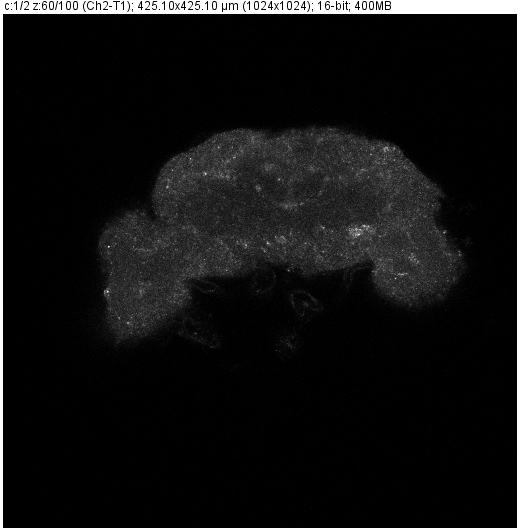
\includegraphics[width=8cm, height=10cm]{in_example}
	\caption{Пример трехмерного двухканального изображения мозга плодовой мушки.}
	\label{in_example}
\end{figure}

\subsection{Получение данных}
Мушки дрозофиллы были выращены при температуре +25 градусов, 12 часов при свете и темноте. 
Каждый исследуемый пол и генотип отбирались из отдельных популяций. Родителям давали 24 часа на откладку яиц.

Во время препарировании отделялась ткань головы и ротовой аппарат, во избежании нанесения повреждений мозгу.

Для исследования использовали дрозофилл поздней стадии (Р15). Дрозофил на поздней стадии куколки легко идентифицировать и препарировать. Также, центральная нервная система мушки на этой стадии и взрослых самцов имеет малые отличия.

\subsection{Оборудование для получения исходных данных}
Образцы были получены постериорно-антериорном направлении с помощью конфокальной системы Zeiss LSM 780 (Carl Zeiss MicroImaging, Inc., Thornwood, NY), объектив: PlanApochromat 20×/1.40.

Конфокальные микроскопы имеют несколько
фотоприемных каналов, что позволяет получить изображения
одновременно в нескольких спектральных диапазонах.  \cite{Inbook}
\begin{figure}[H]
	\centering
	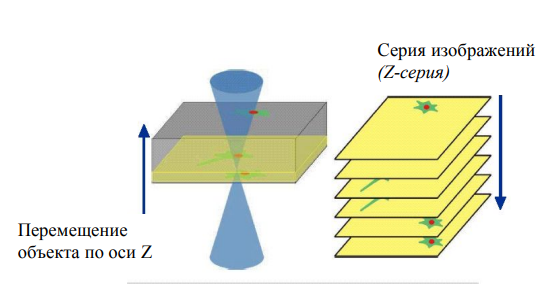
\includegraphics[width=7cm, height=5cm]{z_imgs}
	\caption{Получение серии оптических срезов(Z-серия).}
	\label{z_imgs}
\end{figure}




\section{Сложность задачи} \label{ch1:sec3}
Существует некоторая проблема в решении поставленной задачи. В исходных изображениях наблюдается паразитное свечение из одного канала микроскопа в другом, что вредит выделению частиц. Данное явление называется автофлуоресценцией. Существует несколько методов решения этой проблемы, которые позволяют уменьшить этот эффект, однако конкретный метод и параметры надо тестировать с конкретными изображениями. Также может понадобиться проводить предобработку и модифицировать последующие шаги всей процедуры. 

\section{Существующие методы решений} \label{ch1:sec4}
\begin{figure}[H]
	\centering
	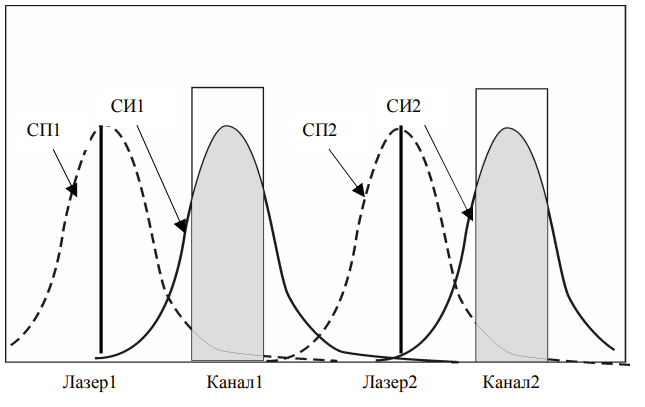
\includegraphics[width=8cm, height=6cm]{c1_c2_norm}
	\caption{Спектры не перекрываются. СП –
		спектры поглощения, СИ – спектры испускания флуорохромов 1 и 2.}
	\label{c1_c2_norm}
\end{figure}

\begin{figure}[H]
	\centering
	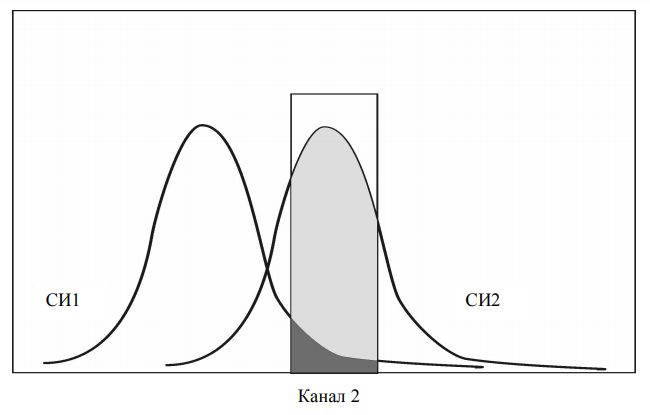
\includegraphics[width=8cm, height=6cm]{c1_c2_bad}
	\caption{Спектры перекрываются слабо.}
	\label{c1_c2_bad}
\end{figure}

\begin{figure}[H]
	\centering
	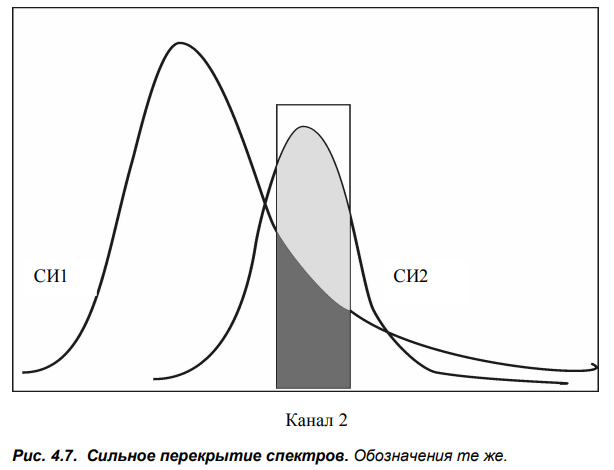
\includegraphics[width=8cm, height=6cm]{c1_c2_baddd}
	\caption{Спектры перекрываются сильно.}
	\label{c1_c2_baddd}
\end{figure}


Рассмотрим все случаи взаимодействия сигналов от
флуорохромов. Отсутствие перекрытия показано на Рис.\ref{c1_c2_norm}. В этом случае можно сканировать одновременно.\cite{Inbook}

Слабое перекрытие спектров на рис. \ref{c1_c2_bad}. Здесь небольшая часть
спектра испускаемого первым флуорохромом попадает в диапазон второго канала. Можно попробовать уменьшить мощность лазера для первого флуорохрома, а также, во избежании потери яркости осуществить сдвиг диапазона приема второго канала правее.\cite{Inbook}

В последнем случаем - когда перекрытие сильное (см. рис. \ref{c1_c2_baddd}) необходимо сканировать последовательно. То есть, сначала включить лазер и фотоприемник только для первого канала и для второго их отключить, затем аналогичено включить для второго и выключить для первого. \cite{Inbook}
 
Также, помимо последовательного сканирования существует вычислительный способ уменьшения перекрытия, основанного различных математических алгоритмах с применением теории по линейной алгебре, математиеской статистике, машинному обучению и статистическому анализу. В данном приёме используется информация о спектрах используемых красителей, значениях интенсивности пикселей изображений.\cite{Inbook} Именно такой способ будет рассмотрен в данной работе.

Наиболее эффективным способом избежания перекрытия спектров является последовательное сканирование, однако у этого подхода есть несколько ограничений.Он требует использования специализированного оборудования и запатентованного программного обеспечения, что является ограничивающим фактором в его широком использовании. Также, например, получения изображений для каждого фотоприемного канала значительно увеличивает время получения изображений и объем данных. \cite{Conference}




%\FloatBarrier % заставить рисунки и другие подвижные (float) элементы остановиться

%% Вспомогательные команды - Additional commands
%
%\newpage % принудительное начало с новой страницы, использовать только в конце раздела
%\clearpage % осуществляется пакетом <<placeins>> в пределах секций
%\newpage\leavevmode\thispagestyle{empty}\newpage % 100 % начало новой страницы